\section{Implementation Details}
\label{sec:imp}
In this section, we summarize the entire algorithm and explain the implemented details.
%
Based on our formulation in Sec.~\ref{sec:method}, our algorithm can be summarized as in Algorithm \ref{alg:jrcs}.
\begin{algorithm}[htb]
	\caption{Joint Registration and Co-segmentation (JRCS)}
	\label{alg:jrcs}
	\textbf{Input:}~~\\
	$\{\vb{V}_m\}$:$M$ 3D point sets\\
	$\Theta^0$:Initial parameters\\
	$\{\beta_{ik}\}_{m}$:layout based prior\\
	\textbf{Output:}~~\\
	$\Theta^q$:Final parameters~~
	\begin{enumerate}
		\item $q\leftarrow1$
		\item \textbf{repeat}
		\item E-step: Use $\Theta^{q-1}$ to estimate $\alpha_{mik}^q$ according to Eq.~(\ref{equ:estep}) (use Eq.~(\ref{equ:bestep}) for a bilateral formulation);
		\item Alter $\alpha_{mik}^q$ with $\{\beta_{ik}\}_{m}$ according to Eq.~(\ref{equ:alteralpha});
		\item M-step-a: use $\alpha^q_{mik}$, $\pmb x^{q-1}_k$ to estimate $\{R_{mn}^q\}$ and $\{\pmb t_{mn}^q\}$ according to Eqs.~(\ref{equ:updateR})(\ref{equ:updatet});
		\item M-step-b: use $\alpha^q_{mik}$, $\{\vb{R}_{mn}^q\}$ and $\{\vb{t}_{mn}^q\}$ to update other parameters for Gaussian models according to Eqs.~ (\ref{equ:updatexk})(\ref{equ:updatesigma})(\ref{equ:updatepk})(\ref{equ:updatey})  (or use Eqs.~ (\ref{equ:updatefk})(\ref{equ:updatefsigma}) for a bilateral formulation);
		\item $q \leftarrow q+1$
		\item \textbf{until} Convergence \cxj{what is the convergence conditions?}
		\item \textbf{return} $\Theta^q$
	\end{enumerate}
\end{algorithm}
\subsection{Implementation Details}
%
\textbf{Initialization of $\Theta$}: We start with determining the total number of Gaussian model $K_{all}$ as we explained in Sec.~\ref{sec:imp:interact}.
We set $p_k=\frac{1}{\sum K_n}$, which means each Gaussian has the same weight at the beginning. 
%
We separate the total $K_{all}$ Gaussian models into $N$ groups to represent $N$ objects. 
%
Each group has $K_n$ Gaussian models based on Eq.~(\ref{equ:K_n}). 
We implement this by recording the start and end indices of the $N$ objects. In other words, we record
$\{0,K_1,K_1+1,K_1+K_2,...,\sum^{N-1}K_n+1,\sum^N K_n\}$. $\{\vb{x}_k\}_n$ are Gaussian centroids of $n^{th}$ group and they are initialized as a random positions uniformly distributed on the surface of a sphere, whose radius $r$ is chosen as the median of the radius of the input point sets. 
%
The center of the $n^{th}$ sphere is $\vb{c}_n=(0,0,z_n)$, where $z_n\in \{-(N-1)r,-(N-3)r,...,(N-1)r\}$.\cxj{What is N? In total, there would be $2N-1$ centers?} \hsy{No, The common difference is $2r$ here. it is $\{-2r,0,2r\}$ when $N=3$ and $\{-3r,-r,r,3r\}$ when $N=4$}
%
This means that the object models are vertically arranged in latent space as shown in Figure~\ref{fig:teaser}(c) and in Figure~\ref{fig:localoptimal}(b). 
We choose vertical arrangement for groups of object merely for the convenience of visualization. \cxj{So you can also set the spheres horizontally or slantly or arbitrarily for registration only?}
%
We choose spheres as the initial shape so that we can initialize all the $\vb{R}_{mn}$ to identity matrix. 
%
For the $\vb{t}_{mn}$ we initialize them as $\vb{t}_{mn}=- \vb{c}_n$ so that all the object model starting with position at origin point when they are transformed to the space of each input set. 
%
However, if the $m^{th}$ input point set has the manually placed layout, we treat the associated $\vb{t}_{mn}$ differently. For this case we have:
\begin{equation}
	\label{equ:initt}
	\vb{t}_{mn}=\frac{\sum_{\vb{v}_{mi} \in B_n}\vb{v}_{mi}}{N(B_n)}-\vb{c}_n
\end{equation}
where $N(B_n)$ here is the number of element in $B_n$ and $B_n$ is the point set that is enclosed by the manually input layout (box) \mdf{indicating arrangement of the $n^{th}$ object}. 
\cxj{You have many boxes, $B_n$ is which one?. The number $n$ is also confusing while you use $n$ for sphere center index.} \hsy{ $n$ is always indices for object and $B_n$ is the box for $n^{th}$ object }
\subsection{Hot Intervention Mechanism}
\cxj{I am curious where do you get this word? Any reference?}
%
Our current implementation of optimization is quite slow (fails to converge in an interactive-rate time) especially when the numbers of points inside the input point sets are large and it is possible for our optimization to stuck in a local optimal, requiring the guide from the manual input. 
%
As a compensation for these drawbacks, we implement a hot intervention mechanism, allowing the manual input to take effect during the optimization process. 
Theoretically, this is possible due to the i.i.d assumption, under which the calculation of posterior probability is independent for each input point set. 
%
Even after the optimization is started, we can still allow the user to add more layouts \cxj{what do you mean by 'add layouts'?} for other point sets and the program can do the same alteration as (\ref{equ:alteralpha}) in the next iteration. 
%
Figure~\ref{fig:hi} shows how the users can use the hot intervention mechanism within our tool.
%
\begin{figure}[htb]
	\centering
	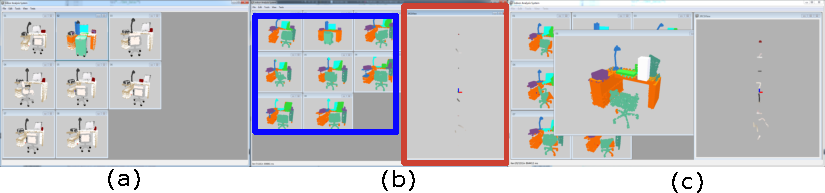
\includegraphics[width=\linewidth]{images/hotintervention/hi}
	\caption{\label{fig:hi} This figure shows the hot intervention mechanism. (a) The input point sets with manually placed layout in the $2^{nd}$ point set. (b) For each iteration, the instant segmentation results for all point sets are shown in the blue region while the object models (the shape of the centroids of the Gaussian models) are shown in the red region. (c) The user picks another input point set and adds more boxes targeting the incorrect segmentation to further guide the optimization when the optimization is running. \cxj{highlight the newly added box. Do not show the entire interface.. just show the data. }}
\end{figure}

